\documentclass[9pt,twocolumn,twoside,]{pnas-new}

% Use the lineno option to display guide line numbers if required.
% Note that the use of elements such as single-column equations
% may affect the guide line number alignment.


\usepackage[T1]{fontenc}
\usepackage[utf8]{inputenc}

% tightlist command for lists without linebreak
\providecommand{\tightlist}{%
  \setlength{\itemsep}{0pt}\setlength{\parskip}{0pt}}


% Pandoc citation processing
\newlength{\cslhangindent}
\setlength{\cslhangindent}{1.5em}
\newlength{\csllabelwidth}
\setlength{\csllabelwidth}{3em}
\newlength{\cslentryspacingunit} % times entry-spacing
\setlength{\cslentryspacingunit}{\parskip}
% for Pandoc 2.8 to 2.10.1
\newenvironment{cslreferences}%
  {}%
  {\par}
% For Pandoc 2.11+
\newenvironment{CSLReferences}[2] % #1 hanging-ident, #2 entry spacing
 {% don't indent paragraphs
  \setlength{\parindent}{0pt}
  % turn on hanging indent if param 1 is 1
  \ifodd #1
  \let\oldpar\par
  \def\par{\hangindent=\cslhangindent\oldpar}
  \fi
  % set entry spacing
  \setlength{\parskip}{#2\cslentryspacingunit}
 }%
 {}
\usepackage{calc}
\newcommand{\CSLBlock}[1]{#1\hfill\break}
\newcommand{\CSLLeftMargin}[1]{\parbox[t]{\csllabelwidth}{#1}}
\newcommand{\CSLRightInline}[1]{\parbox[t]{\linewidth - \csllabelwidth}{#1}\break}
\newcommand{\CSLIndent}[1]{\hspace{\cslhangindent}#1}


\templatetype{pnasresearcharticle}  % Choose template

\title{Les scientifiques sont-ils crédibles ?}

\author[a,1]{Jordan Lenneville}

  \affil[a]{Université de Sherbrooke, Écologie, 2500 bd de l'Université,
Sherbrooke, Qc, J1K 2R1}


% Please give the surname of the lead author for the running footer
\leadauthor{Lenneville}

% Please add here a significance statement to explain the relevance of your work
\significancestatement{Cet article a été rédigé dans le cadre du cours
de Méthodes en écologie computationnelle (BIO500). Ce travail à comme
but de formuler et défendre une opinion sur les enjeux de
reproductibilité en écologie. Plus précisément, les élèves sont mendatés
à s'exprimer sur l'importance de la transparence et des standards de
reproductibilité dans un contexte où il y a une accélération de la
recherche.}


\authorcontributions{}



\correspondingauthor{\textsuperscript{1} E-mail:
\href{mailto:lenj0501@USherbrooke.ca}{\nolinkurl{lenj0501@USherbrooke.ca}}}

% Keywords are not mandatory, but authors are strongly encouraged to provide them. If provided, please include two to five keywords, separated by the pipe symbol, e.g:
 \keywords{  Reproductibilité |  Transparence |  BDPM  } 

\begin{abstract}
La crise de reproductibilité se fait de plus en plus sentir dans la
science. De nombreux scientifiques sont incapables de reproduire
différentes expériences incluant les leurs. 34\% des chercheurs n'ont
même pas de procédures établies pour assurer un minimum de
reproductibilité (1). Les scientifiques modernes ont-ils perdu leur
crédibilité ? La science recherche-t-elle encore la vérité ou est-elle
plutôt à la chasse aux résultats ? Chose sûre la communauté scientifique
manque de transparence dans leurs publications, mais plusieurs sont
poussé à publier précocement. Il n'existe probablement pas de remède
miracle à cette crise, mais ils existent certainement quelques solutions
pour améliorer la situation telle que le Broad Daylight Publication
Model (BDPM) (2).
\end{abstract}

\dates{This manuscript was compiled on \today}
\doi{\url{www.pnas.org/cgi/doi/10.1073/pnas.XXXXXXXXXX}}

\begin{document}

% Optional adjustment to line up main text (after abstract) of first page with line numbers, when using both lineno and twocolumn options.
% You should only change this length when you've finalised the article contents.
\verticaladjustment{-2pt}



\maketitle
\thispagestyle{firststyle}
\ifthenelse{\boolean{shortarticle}}{\ifthenelse{\boolean{singlecolumn}}{\abscontentformatted}{\abscontent}}{}

% If your first paragraph (i.e. with the \dropcap) contains a list environment (quote, quotation, theorem, definition, enumerate, itemize...), the line after the list may have some extra indentation. If this is the case, add \parshape=0 to the end of the list environment.

\acknow{Merci Dominique pour ce cours qui m'a été utile pour optimiser
mon temps de codage. J'ai surtout aimer travailler avec Rmarkdown. Bon
été!

\textbf{Bibliographie}}

\hypertarget{introduction}{%
\section*{Introduction}\label{introduction}}
\addcontentsline{toc}{section}{Introduction}

Le questionnement de la crédibilité des scientifiques, que ce soit pour
leur reproductibilité ou leur transparence, est de plus en plus
populaire. En effet, comme mentionné dans l'étude de Fanelli (3),
l'augmentation d'article dédié à ce sujet, au cours des dernières
années, est exponentielle (Fig 1). Le sondage fait par Baker (1) a amené
plusieurs réponses assez inquiétantes. En effet,70\% des chercheurs
interrogés ont déjà échoué à reproduire des expériences effectuées
d'autres chercheurs et plus de la moitié d'entre eux ont échoué à
reproduire leur(s) propre(s) expérience(s). Finalement, toujours selon
le sondage de Bake (1), 52\% des scientifiques interrogés croient qu'il
y a une crise majeure de reproductibilité au sein de leur communauté.
Ces sondages ont alors amené plusieurs scientifiques à se pencher sur le
sujet de la reproductibilité et de la transparence afin de découvrir
quels sont les différents problèmes qui nous a amenés à cette crise et
quelles sont les solutions. Avant de se lancer sur les différents
problèmes et solutions de ce sujet il est important d'avoir une
définition générale de la reproductibilité et la transparence. Tout
d'abord, il n'existe pas de définition précise pour la reproductibilité,
car la variété qui se retrouve dans les différents sujets scientifiques
est énorme (4). C'est pourquoi qu'il est normal de n'être pas capable de
reproduire chaque détail d'une expérience effectuée ultérieurement (4).
Toutefois, le minimum de reproductibilité qui devrait être atteignable
est d'arrivée aux mêmes grandes conclusions du départ lorsqu'on
reproduit une expérience (4). La transparence est aussi un sujet n'ayant
pas de définition précise. Toutefois, un article dédié à la taxonomie de
la transparence en science (5), a recensé les différents concepts de
transparence amenés par les scientifiques et les a séparés en 8
dimensions qu'on peut retrouver à cette figure (Fig 2).

\hypertarget{argumentation}{%
\section*{Argumentation}\label{argumentation}}
\addcontentsline{toc}{section}{Argumentation}

\hypertarget{probluxe8mes}{%
\subsection*{Problèmes}\label{probluxe8mes}}
\addcontentsline{toc}{subsection}{Problèmes}

Énormément de problèmes ont été recensés comme étant la cause de cette
crise de reproductibilité. Évidemment, certains problèmes sont jugés
plus importants que d'autres. Par exemple, il a été mentionné que les
environnements très contrôlés, que sont les laboratoires, empêchent de
reproduire les mêmes résultats, car les facteurs environnementaux qui
sont spécifiques à chaque laboratoire sont très difficiles à reproduire
(6). Un autre problème majeur serait que beaucoup d'articles font de la
sélection de résultats, c'est-à-dire de démontrer seulement les
résultats qui sont en faveur de leurs hypothèses et d'omettre de
présenter les résultats qui ne sont pas significatifs (7), (1). D'autres
scientifiques croient que ce sont les faibles analyses et forces
statistiques qui empêchent beaucoup d'études d'être reproductible (3),
(1), (8). En effet, ce problème ferait en sorte qu'il y a beaucoup plus
de chances d'avoir un faux positif (3) et donc d'avoir un problème
statistique de type 2 qui consiste à ne pas rejeter l'hypothèse
lorsqu'elle est fausse (8). Personnellement, je crois que les problèmes
expliquant le mieux le manque de reproductibilités sont la pression de
publier de plus en plus vite et le manque flagrant de transparence.
Récemment avec la Covid, il a été observé que la pression pour publier
était forte (9). De plus, à cause de la pandémie et la pression de
publier, des exceptions ont été acceptées afin de diminuer les standards
de qualité normaux (appelées \textless{}\textgreater) (9) et ainsi
augmenter la vitesse de publication. Cela fait en sorte que ces études
obtiennent des résultats beaucoup plus rapides que les études
rigoureuses, et reçoivent donc plus de subventions même si la plupart de
ces publications non rigoureuses obtiennent des résultats faussement
positifs (9). Il a également été observer qu'avec une forte pression de
publication, les scientifiques sont plus enclins à faire de la fraude
(10). Il est normal de croire que le manque de transparence des
publications scientifiques cause un manque de reproductibilité. En
effet, le manque de publication de données d'un projet et le secret du
processus de la révision par les pairs est problématiques puisqu'il est
beaucoup plus difficile de vraiment savoir s'il y a de la fraude et/ou
des erreurs de statistiques dans les données (2). De plus, en
\textless{}\textgreater{} le processus de révision des pairs il est
impossible de savoir la qualité de la révision (2).

\hypertarget{solutions}{%
\subsection*{Solutions}\label{solutions}}
\addcontentsline{toc}{subsection}{Solutions}

Plusieurs solutions ont été proposées pour les différents problèmes
mentionnés précédemment. Toutefois, je crois que la meilleure solution
est une transparence améliorée, mais contrôlée. Je dis contrôlé, car
plusieurs scientifiques sont réticents à être 100\% transparents et ils
ont de bons arguments. En effet, les longues études qui s'étalent sur de
nombreuses années pourraient être grandement touchées par une
transparence totale (11). Dans cet article, il est mentionné que la
majorité des scientifiques responsables de longues études sont inquiets
de fournir leurs données au public pour plusieurs raisons (11). 1-
puisque les données et méthodes des longues études sont très complexes
il est fort probable qu'ils seront interprétés d'une mauvaise manière
par le public. 2- Il risque d'avoir moins de collaborations, car il ne
serait plus nécessaire d'être collaborateurs pour avoir accès aux
données. 3- Les études à long terme risque d'avoir encore plus de
difficultés à se subventionner, déjà que la plupart d'entre eux font
face à des problèmes de subventions (Fig 3) (11). Selon moi, la
meilleure solution pour avoir une transparence contrôlée qui optimise la
reproductibilité serait la solution proposée dans cette étude (2). Leur
système se nomme Broad Daylight Publication Model (BDPM) et contient
trois volets principaux : 1- la transparence du processus éditorial 2-
la responsabilité des réviseurs 3- l'ouverture des données au public
avec un certain contrôle. Leur premier volet consiste à rendre publiques
toutes demandes (acceptées refusées) pour être publiés dans les
différents journaux. Ce volet consiste également à rendre publiques
toutes les revues des différents articles. Leur deuxième volet consiste
à permettre aux lecteurs d'attribuer des cotes aux réviseurs en fonction
de leur travail de révision. Cela fera en sorte que le système de
révision sera optimal, car les mauvais réviseurs auront une mauvaise
cote et les chercheurs seront donc moins enclins de les prendre dans
leurs prochaines études. Finalement, le troisième assure un contrôle de
la transparence par une confidentialité des participants aux études et
par un moratoire d'une durée déterminée qui pourra être établi pour les
études de longue durée. Cela donne donc une longueur d'avance aux
chercheurs originaux d'une étude afin d'éviter qu'ils soient dépassés
par d'autres équipes de chercheurs qui pourraient avoir accès à leurs
données.

\hypertarget{conclusion}{%
\section*{Conclusion}\label{conclusion}}
\addcontentsline{toc}{section}{Conclusion}

Pour résumer, les recherches sont de plus en plus contestées, car elles
présentent un grand problème de reproductibilités. Les raisons qui
pourraient expliquer cette crise sont assez variées. Certains croient
que ce serait le manque de variabilité dans les échantillons analysés,
d'autres croient que ce seraient des statistiques faibles et remplies
d'erreurs. Toutefois, je crois que les raisons principales dernières
cette crise sont la pression de publier et le manque de transparence. La
meilleure façon de régler ces problèmes serait d'employer le BDPM
puisque ce modèle améliore le système de révision par les pairs et
permet d'avoir un contrôle de la transparence qui supporte les études de
longue durée. Ce modèle pourrait même régler le problème de pression de
publication, car les bons réviseurs n'accepteront pas des études qui ne
sont pas rigoureuses dans leur méthode.

\begin{figure}
\centering
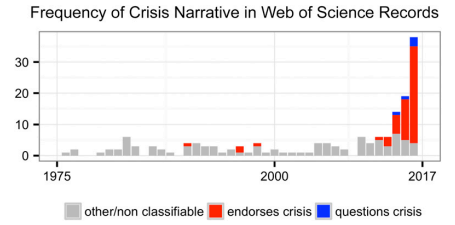
\includegraphics[width=0.5\textwidth,height=0.5\textheight]{image intro .png}
\caption{L'augmentation d'articles dédiés à la crise de
reproductibilité}
\end{figure}

\begin{figure}
\centering
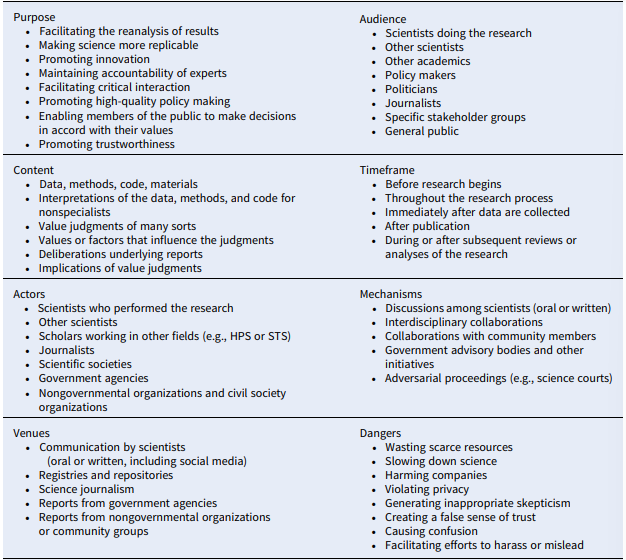
\includegraphics[width=0.5\textwidth,height=0.4\textheight]{Transparence.png}
\caption{Les 8 dimensions de la transparence}
\end{figure}

\begin{figure}
\centering
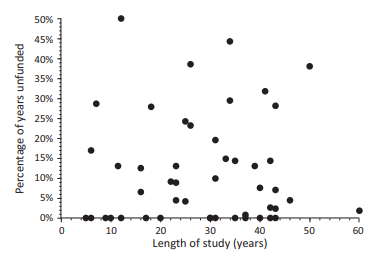
\includegraphics[width=0.4\textwidth,height=0.4\textheight]{Subventions.png}
\caption{Durée de l'étude et pourcentage d'années non subventionnées}
\end{figure}

\showmatmethods
\showacknow
\pnasbreak

\hypertarget{refs}{}
\begin{CSLReferences}{0}{0}
\leavevmode\vadjust pre{\hypertarget{ref-baker_1500_2016}{}}%
\CSLLeftMargin{1. }
\CSLRightInline{Baker M (2016) 1,500 scientists lift the lid on
reproducibility. \emph{Nature} 533(7604):452--454.}

\leavevmode\vadjust pre{\hypertarget{ref-wicherts_letting_2012}{}}%
\CSLLeftMargin{2. }
\CSLRightInline{Wicherts J, Kievit R, Bakker M, Borsboom D (2012)
Letting the daylight in: {Reviewing} the reviewers and other ways to
maximize transparency in science. \emph{Frontiers in Computational
Neuroscience} 6. Available at:
\url{https://www.frontiersin.org/article/10.3389/fncom.2012.00020}
{[}Accessed April 23, 2022{]}.}

\leavevmode\vadjust pre{\hypertarget{ref-fanelli_is_2018}{}}%
\CSLLeftMargin{3. }
\CSLRightInline{Fanelli D (2018) Is science really facing a
reproducibility crisis, and do we need it to? \emph{Proceedings of the
National Academy of Sciences} 115(11):2628--2631.}

\leavevmode\vadjust pre{\hypertarget{ref-begley_reproducibility_2015}{}}%
\CSLLeftMargin{4. }
\CSLRightInline{Begley CG, Ioannidis JPA (2015) Reproducibility in
{Science}. \emph{Circulation Research} 116(1):116--126.}

\leavevmode\vadjust pre{\hypertarget{ref-elliott_taxonomy_2020}{}}%
\CSLLeftMargin{5. }
\CSLRightInline{Elliott KC (2020) A {Taxonomy} of {Transparency} in
{Science}. \emph{Canadian Journal of Philosophy}:1--14.}

\leavevmode\vadjust pre{\hypertarget{ref-milcu_genotypic_2018}{}}%
\CSLLeftMargin{6. }
\CSLRightInline{Milcu A, et al. (2018) Genotypic variability enhances
the reproducibility of an ecological study. \emph{Nature Ecology \&
Evolution} 2(2):279--287.}

\leavevmode\vadjust pre{\hypertarget{ref-saini_selective_2014}{}}%
\CSLLeftMargin{7. }
\CSLRightInline{Saini P, et al. (2014) Selective reporting bias of harm
outcomes within studies: Findings from a cohort of systematic reviews.
\emph{BMJ} 349:g6501.}

\leavevmode\vadjust pre{\hypertarget{ref-nakagawa_farewell_2004}{}}%
\CSLLeftMargin{8. }
\CSLRightInline{Nakagawa S (2004) A farewell to {Bonferroni}: The
problems of low statistical power and publication bias. \emph{Behavioral
Ecology} 15(6):1044--1045.}

\leavevmode\vadjust pre{\hypertarget{ref-london_against_2020}{}}%
\CSLLeftMargin{9. }
\CSLRightInline{London AJ, Kimmelman J (2020) Against pandemic research
exceptionalism. \emph{Science} 368(6490):476--477.}

\leavevmode\vadjust pre{\hypertarget{ref-eisner_reproducibility_2018}{}}%
\CSLLeftMargin{10. }
\CSLRightInline{Eisner DA (2018) Reproducibility of science: {Fraud},
impact factors and carelessness. \emph{Journal of Molecular and Cellular
Cardiology} 114:364--368.}

\leavevmode\vadjust pre{\hypertarget{ref-mills_archiving_2015}{}}%
\CSLLeftMargin{11. }
\CSLRightInline{Mills JA, et al. (2015) Archiving {Primary} {Data}:
{Solutions} for {Long}-{Term} {Studies}. \emph{Trends in Ecology \&
Evolution} 30(10):581--589.}

\end{CSLReferences}



% Bibliography
% \bibliography{pnas-sample}

\end{document}
